\section{Results} \label{sec:results}
The results presented in the following are based on simulations performed using the commercial simulator~\cite{questa}. The output logs were then post-processed with custom \emph{tcl} scripts, run within the simulator shell, and with \textsc{matlab} scripts.

\subsection{\acl{alu}}

\begin{figure}
    \centering
    \subfloat[][The histogram shows that the applied stimulus was effective for exercising
    all the operations supported by the \ac{dut}. The \emph{funclsr} is faulty, having generated wrong results in $1/3$ of the cases.\label{fig:alu_op}]
        {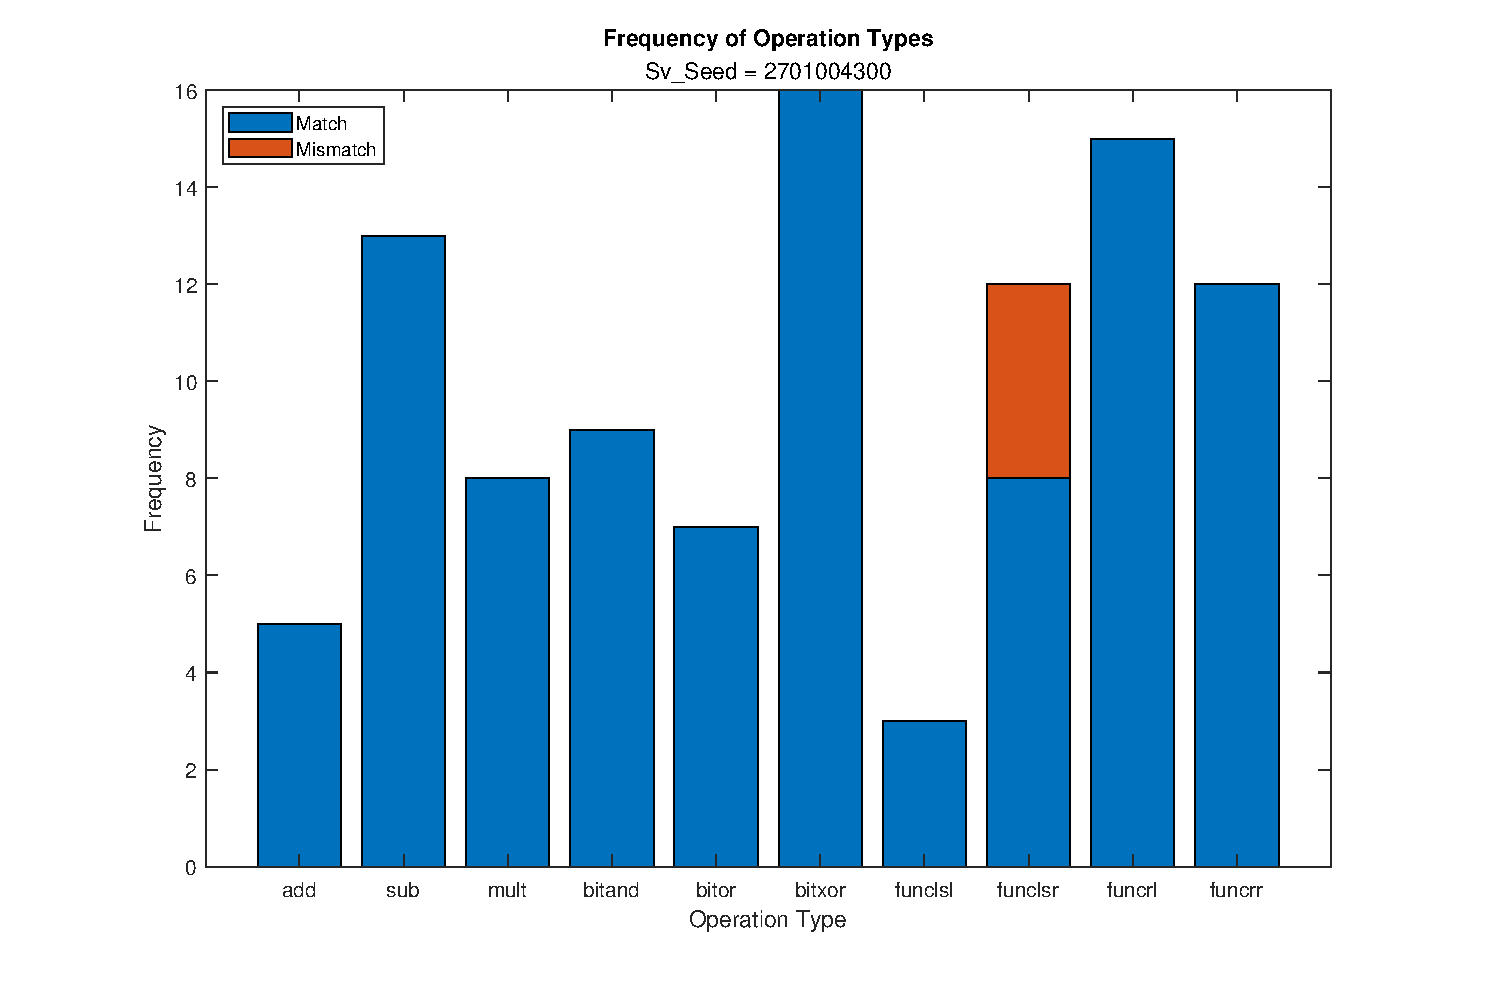
\includegraphics[width=.8\textwidth]{fig/alu_opdist.eps}} \\
    \subfloat[][This bar plot allows us to appreciate how the realizations of the input operands are distributed in the support set. In compliance with the chosen weighted distribution, the stimulus is skewed towards the corner cases: this is where the 4 errors of the \emph{funclsr} operation are located.\label{fig:alu_ab}]
        {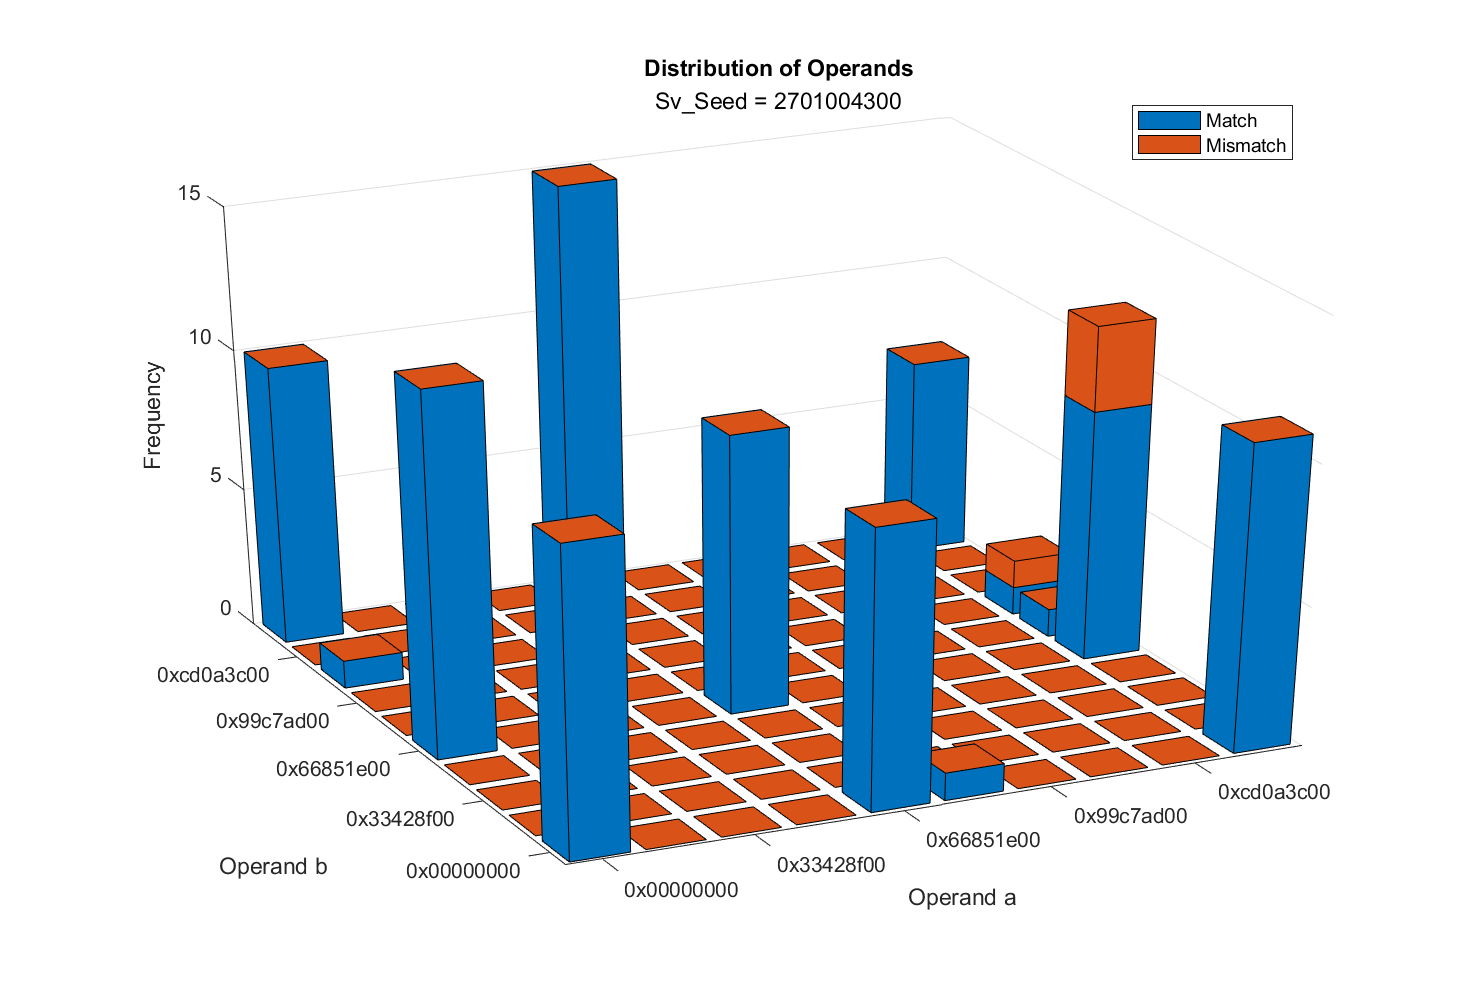
\includegraphics[width=\textwidth]{fig/alu_abdist.eps}}
    \caption{Visualization of the simulation logs for the \ac{alu} under test: \qty{32}{\bit} parallelism, \num{100} packets.}
    \label{fig:alu}
\end{figure}

\begin{figure}
    \centering
    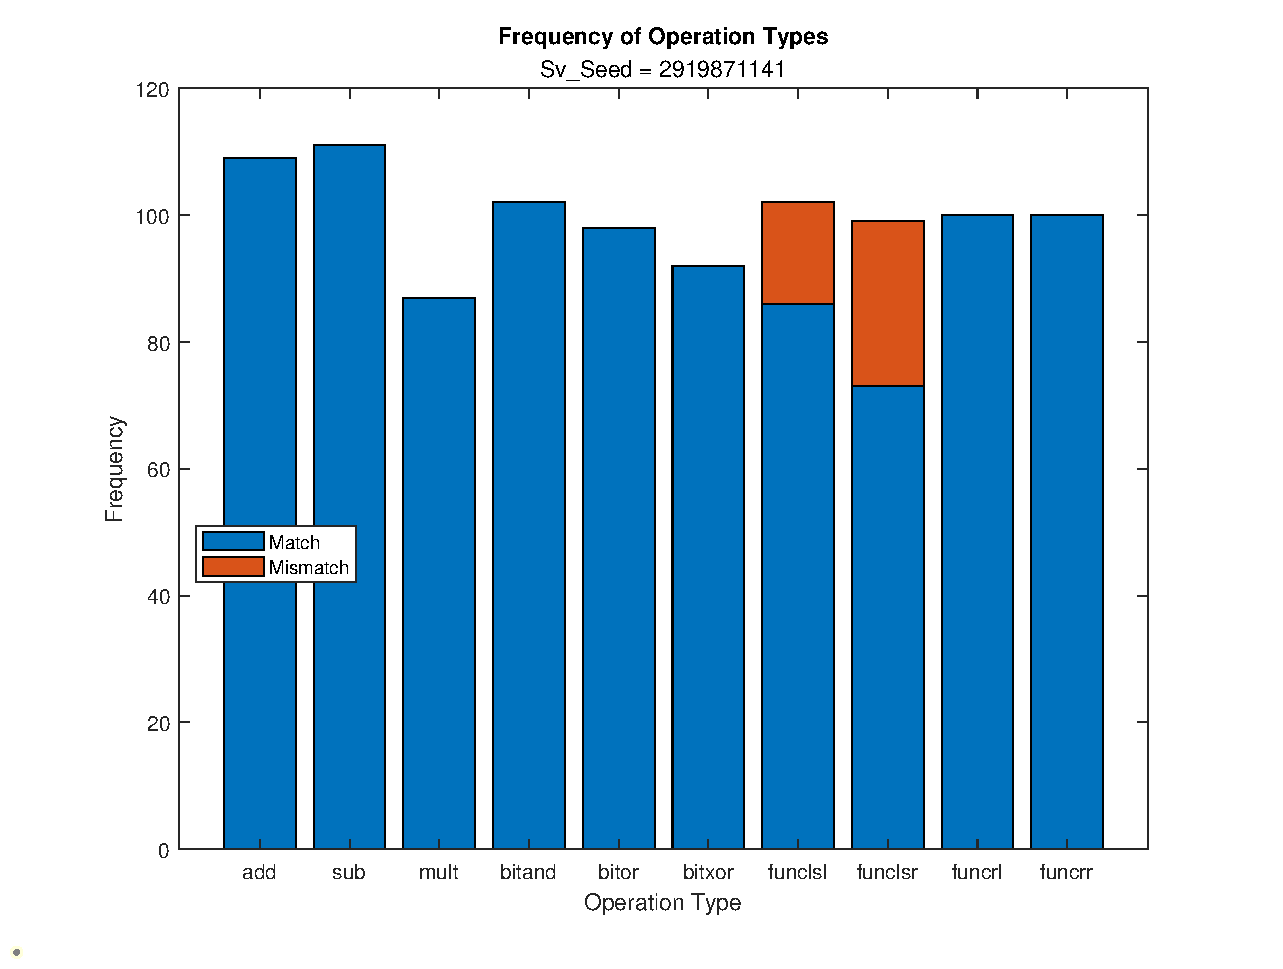
\includegraphics[width=.8\textwidth]{fig/alu_opdist_1000.eps}
    \caption{Additional run of the \ac{alu} simulation: \qty{32}{\bit} parallelism, \num{1000} packets. Both \emph{funclsr} and \emph{funclsl} are faulty.}
    \label{fig:alu_1000}
\end{figure}

The \ac{alu} was initially tested using a random seed, data parallelism of \qty{32}{\bit} and \num{100} packets. The simulation log prints:
\begin{minted}[bgcolor=mintedbackground, fontsize=\scriptsize]{text}
# @1010: Scoreboard: 100 expected packets, 100 received packets
# 
# @1010: END OF SIMULATION
#          * 4 error(s)
#          * total functional coverage: 100.00%
\end{minted}
The representation of the output is in~\cref{fig:alu}. 

Impersonating both the design team and the verification team, the additional knowledge about the \ac{rtl} description gives an advantage in the understanding of what could have gone wrong. Before that, I can highlight a first shortcoming in the definition of the cover group: it would be very useful to have an insight into the distribution of the operand corner cases per operation type. Otherwise, I would have to compute them in post-processing. 

Doubting that the stimulus was sufficient to exercise all operation types in the corner cases, I repeated the simulation increasing the packets number to \num{1000}; the results in~\cref{fig:alu_1000} prove that both \emph{funclsr} and \emph{funclsl} are faulty.

\subsubsection{Debugging}
Looking at the offending lines in the behavioral description of the \ac{alu}:
\begin{minted}[bgcolor=mintedbackground, fontsize=\scriptsize]{vhdl} 
when funclsl =>
    outalu <= std_logic_vector(shift_left(unsigned(data1), to_integer(unsigned(data2))));
when funclsr =>
    outalu <= std_logic_vector(shift_right(unsigned(data1), to_integer(unsigned(data2))));
\end{minted}
I observe that the second operand is not sliced to restrict the maximum number of shift locations inside \svinline{[0:data_width-1]}. Now, looking at the details in the simulation log for one of such errors:
\begin{minted}[bgcolor=mintedbackground, fontsize=\scriptsize]{text} 
# ** Warning: (vsim-151) NUMERIC_STD.TO_INTEGER: Value -2 is not in bounds of subtype NATURAL.
#    Time: 10 ns  Iteration: 2  Instance: /alu_top/dut/alu_i
# @20: Monitor: Packet id=2: { r=fffffffe }
# @20: Scoreboard: check: Packet id=2: { r=fffffffe }
#                  against: Packet id=1: { a=7fffffff, b=ffffffff, r=00000000, op=funclsr }
#                  ERROR MISMATCH
\end{minted}
Searching the \texttt{ieee} library\footnote{\texttt{Revision: \#1, Date: 2020/10/03}}, the function that gets called is:
\begin{minted}[bgcolor=mintedbackground, fontsize=\scriptsize]{vhdl} 
  -- Id: D.1
  function TO_INTEGER (ARG : UNRESOLVED_UNSIGNED) return NATURAL is
    constant ARG_LEFT : INTEGER := ARG'length-1;
    alias XXARG       : UNRESOLVED_UNSIGNED(ARG_LEFT downto 0) is ARG;
    variable XARG     : UNRESOLVED_UNSIGNED(ARG_LEFT downto 0);
    variable RESULT   : NATURAL := 0;
  begin
    if (ARG'length < 1) then
      assert NO_WARNING
        report "NUMERIC_STD.TO_INTEGER: null detected, returning 0"
        severity warning;
      return 0;
    end if;
    XARG := TO_01(XXARG, 'X');
    if (XARG(XARG'left) = 'X') then
      assert NO_WARNING
        report "NUMERIC_STD.TO_INTEGER: metavalue detected, returning 0"
        severity warning;
      return 0;
    end if;
    for I in XARG'range loop
      RESULT := RESULT+RESULT;
      if XARG(I) = '1' then
        RESULT := RESULT + 1;
      end if;
    end loop;
    return RESULT;
  end function TO_INTEGER;
\end{minted}
The problem originates from the conversion loop: the underlying data type is not wide enough, therefore \vhdlinline{to_integer(X"ffffffff")} conversion fails to return \num{4294967295}. In fact, the package \texttt{standard}\footnote{VHDL 2008 Language Reference Manual} defines:
\begin{minted}[bgcolor=mintedbackground, fontsize=\scriptsize]{vhdl} 
type INTEGER is range -2147483648 to 2147483647;
subtype NATURAL is INTEGER range 0 to INTEGER'HIGH;
\end{minted}

\subsection{Accumulator}

\begin{figure}
    \centering
    \subfloat[][The bar plot highlights that no violations occurred; as in the case of the \ac{alu}, input operands are localized in the corner cases.\label{fig:acc_ab}]
        {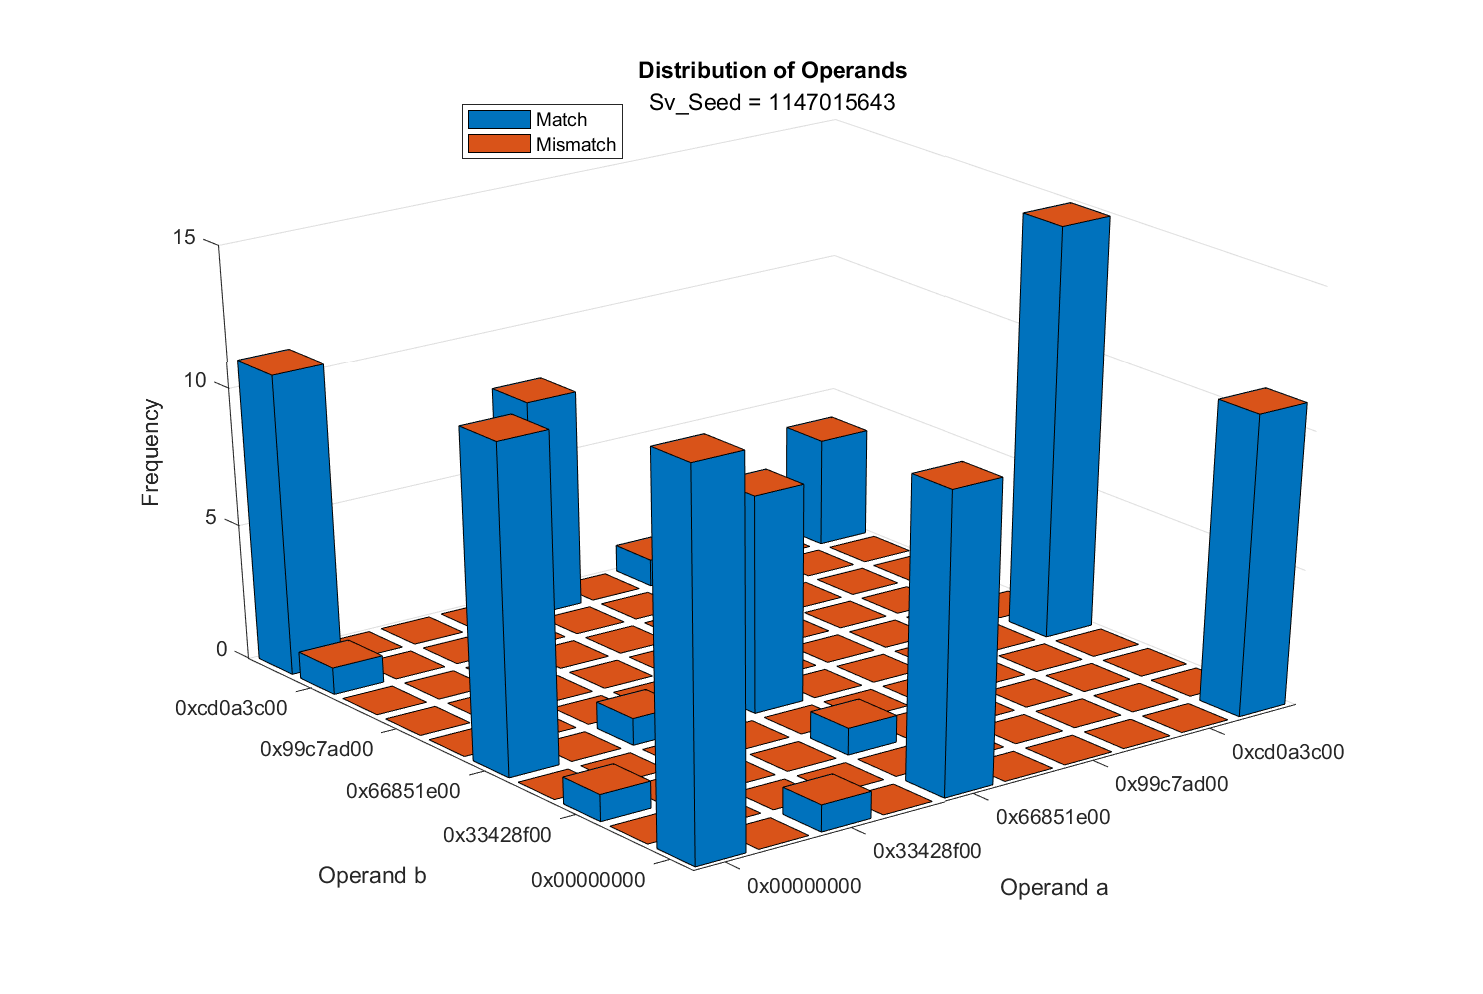
\includegraphics[width=\textwidth]{fig/acc_abdist.eps}}\\
    \subfloat[][In the pie chart we can observe the relative time the \ac{dut} spent in each one of the possible states.\label{fig:acc_state}]
        {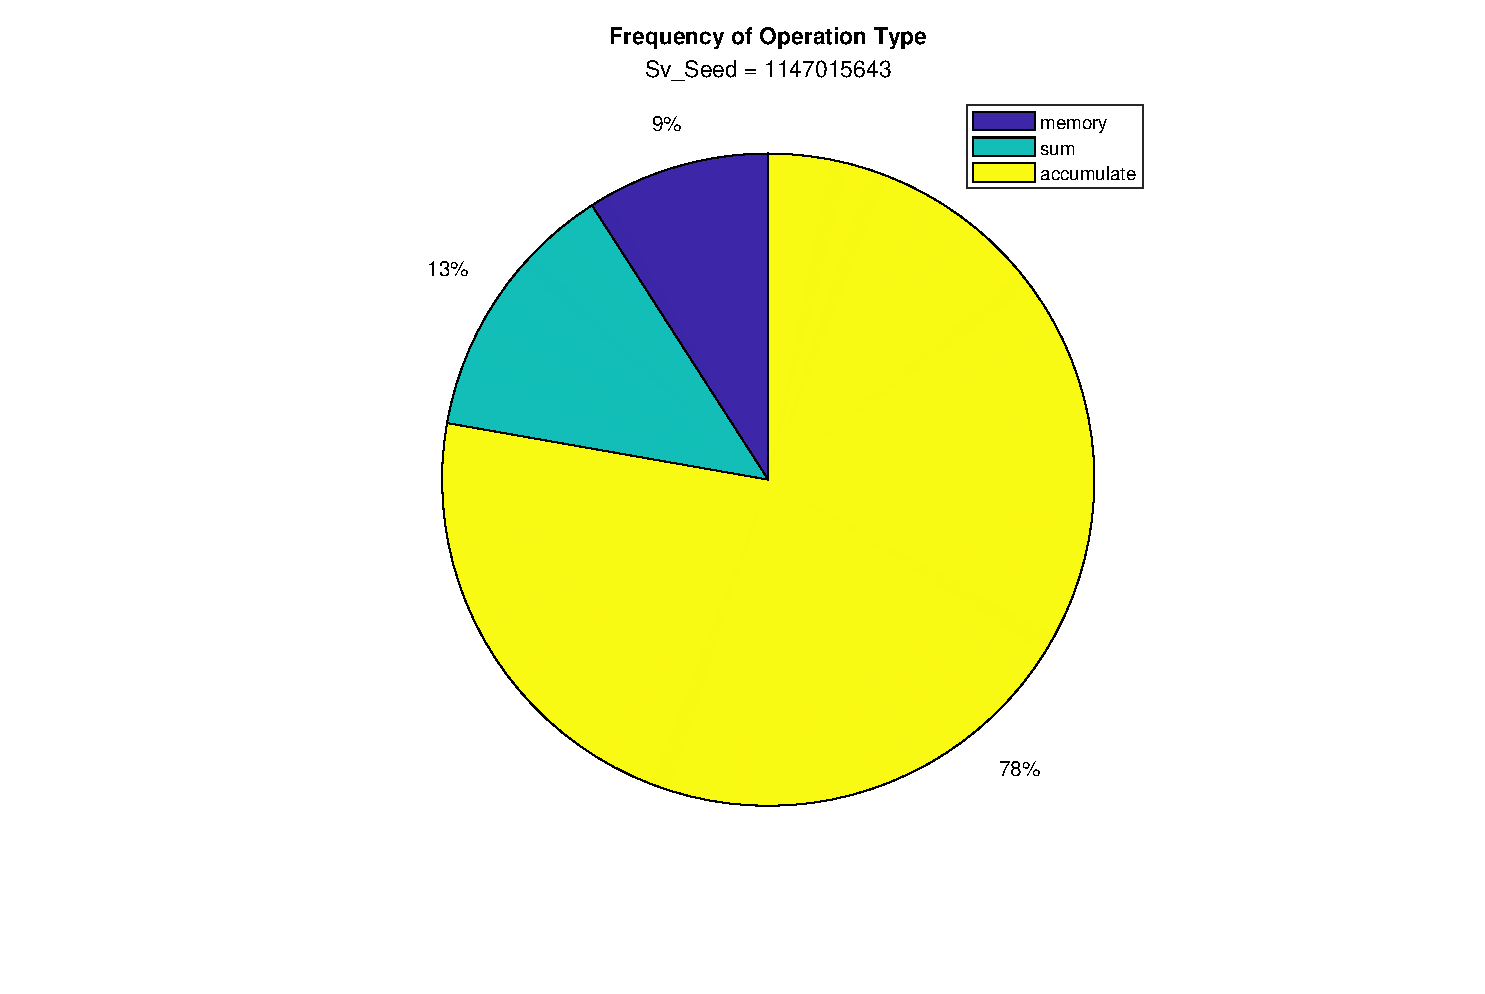
\includegraphics[width=.8\textwidth]{fig/acc_statedist.eps}}
    \caption{Visualization of the simulation logs for the accumulator under test; \qty{32}{\bit} parallelism, 100 packets.}
    \label{fig:acc}
\end{figure}

 Similarly, the accumulator was initially tested using a random seed, data parallelism of \qty{32}{\bit} and \num{100} packets. The simulation log prints:
\begin{minted}[bgcolor=mintedbackground, fontsize=\scriptsize]{text}
# @1020: Scoreboard: 100 expected packets, 100 received packets
# 
# @1020: END OF SIMULATION
#          * 0 error(s)
#          * total functional coverage: 100.00%
\end{minted}
The representation of the output is in~\cref{fig:acc}. Specifically, the cross-coverage data is represented in the pie chart of~\cref{fig:acc_state} and allows us to appreciate how long the \ac{dut} operated in its different states. On the other hand, \cref{fig:acc_ab} highlights how the weighted distribution constraint effectively skewed the stimulus towards the boundaries of the support set.